% $Header: /Users/joseph/Documents/LaTeX/beamer/solutions/conference-talks/conference-ornate-20min.en.tex,v 90e850259b8b 2007/01/28 20:48:30 tantau $

\documentclass{beamer}

% This file is a solution template for:

% - Talk at a conference/colloquium.
% - Talk length is about 20min.
% - Style is ornate.



% Copyright 2004 by Till Tantau <tantau@users.sourceforge.net>.
%
% In principle, this file can be redistributed and/or modified under
% the terms of the GNU Public License, version 2.
%
% However, this file is supposed to be a template to be modified
% for your own needs. For this reason, if you use this file as a
% template and not specifically distribute it as part of a another
% package/program, I grant the extra permission to freely copy and
% modify this file as you see fit and even to delete this copyright
% notice. 


\mode<presentation>

\usepackage[english]{babel}
\usepackage{graphicx}
\usepackage[latin1]{inputenc}
\usepackage{times}
\usepackage[T1]{fontenc}


\title[Short Paper Title] % (optional, use only with long paper titles)
{Deep Exponential Families: Biologically-Plausible Hierarchical Bayesian Inference?}

\author[Author] % (optional, use only with lots of authors)
{David Halpern}


\institute[NYU] % (optional, but mostly needed)
{Department of Psychology\\
  New York University}
% - Use the \inst command only if there are several affiliations.
% - Keep it simple, no one is interested in your street address.

\date[OCNC] % (optional, should be abbreviation of conference name)
{OIST Computational Neuroscience Course 2015}

% If you have a file called "university-logo-filename.xxx", where xxx
% is a graphic format that can be processed by latex or pdflatex,
% resp., then you can add a logo as follows:

\pgfdeclareimage[height=0.5cm]{university-logo}{gsas_long_color.png}
\logo{\pgfuseimage{university-logo}}

\begin{document}

\begin{frame}
  \titlepage
\end{frame}

% Structuring a talk is a difficult task and the following structure
% may not be suitable. Here are some rules that apply for this
% solution: 

% - Exactly two or three sections (other than the summary).
% - At *most* three subsections per section.
% - Talk about 30s to 2min per frame. So there should be between about
%   15 and 30 frames, all told.

% - A conference audience is likely to know very little of what you
%   are going to talk about. So *simplify*!
% - In a 20min talk, getting the main ideas across is hard
%   enough. Leave out details, even if it means being less precise than
%   you think necessary.
% - If you omit details that are vital to the proof/implementation,
%   just say so once. Everybody will be happy with that.

\begin{frame}{Background}
 \begin{columns}[T]
    \begin{column}{.5\textwidth}
  	\begin{itemize}
  	\item
    	Humans and animals have been shown to perform near optimal hierarchical Bayesian inference in a wide variety of perceptual and cognitive tasks
  	\begin{itemize}
    	\item
   		But analytic computation of full posterior is often intractable and must be approximated   
   	\end{itemize}
  	\item
    	What plausible neural algorithms could support this?
   	\end{itemize}	
    \end{column}
    \begin{column}{.5\textwidth}
    	    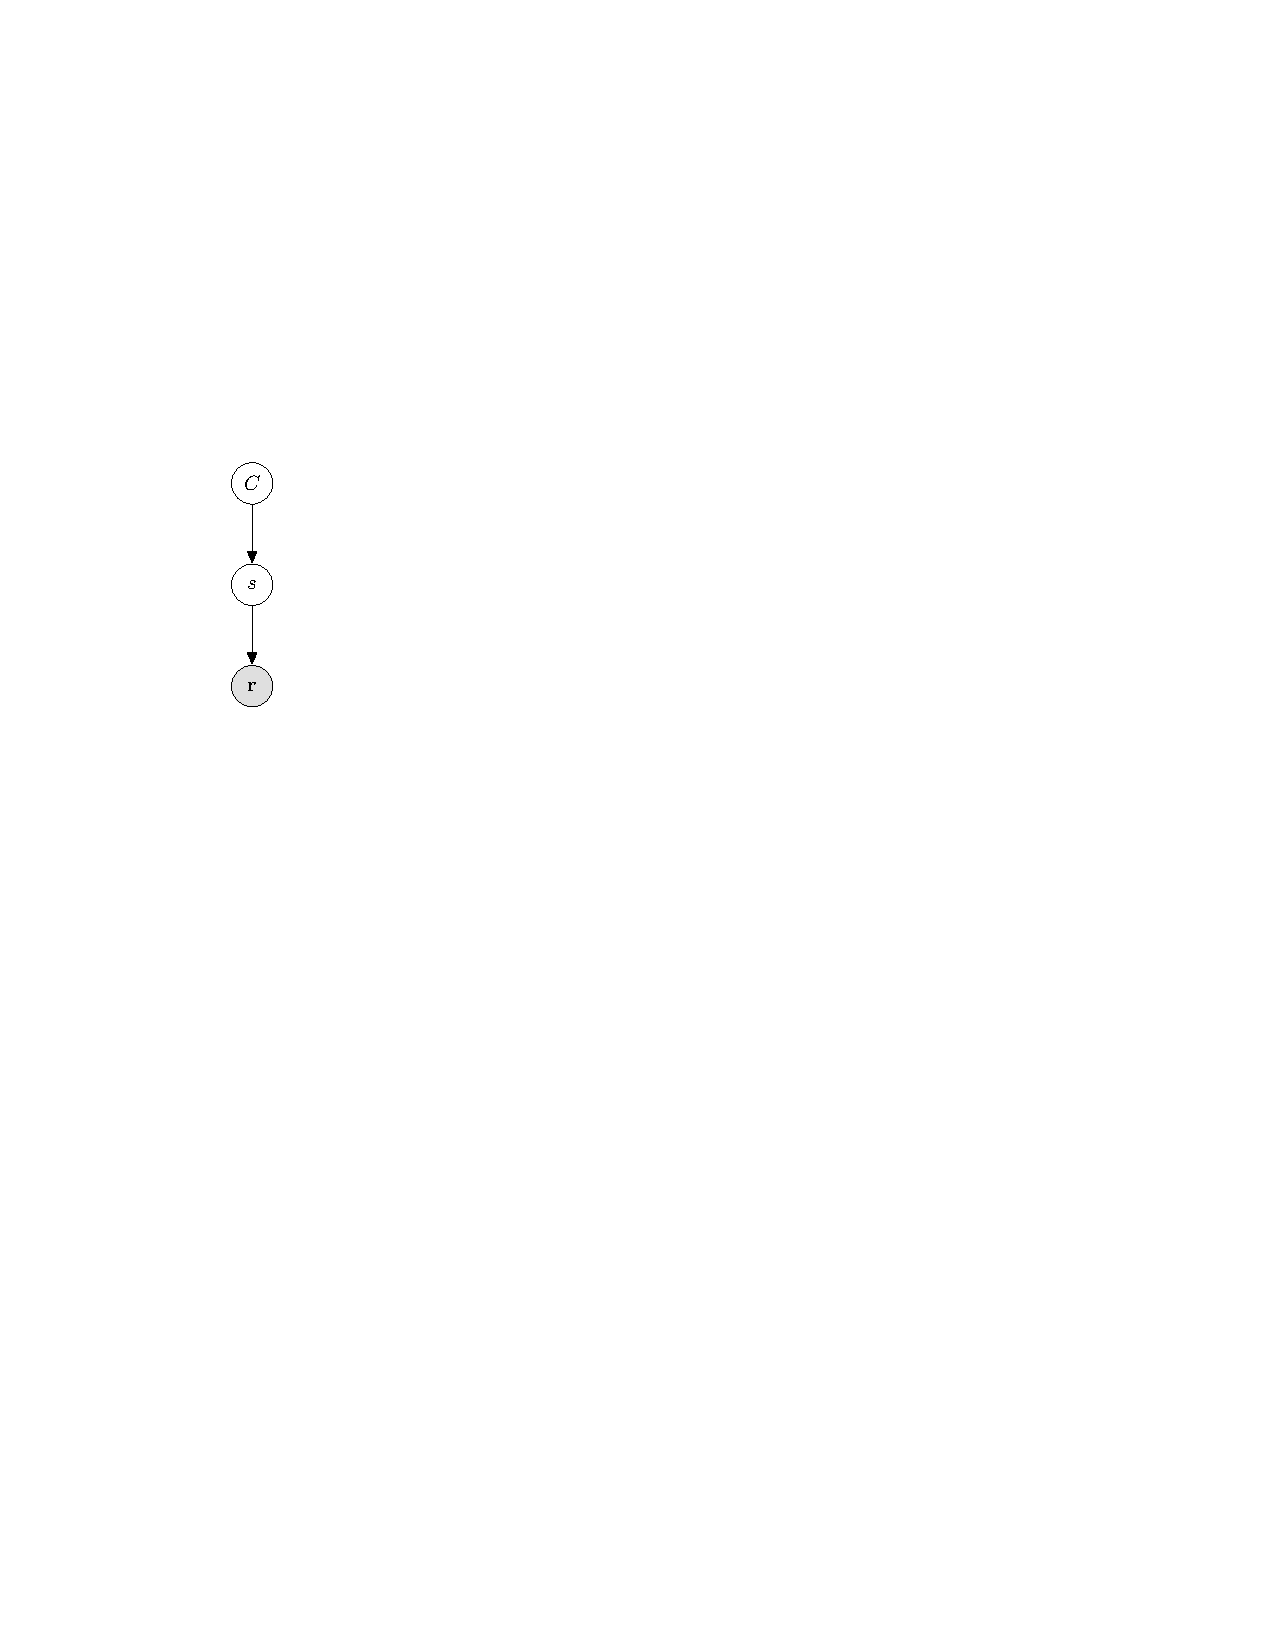
\includegraphics[width = .2\textwidth]{GM.pdf}
   	    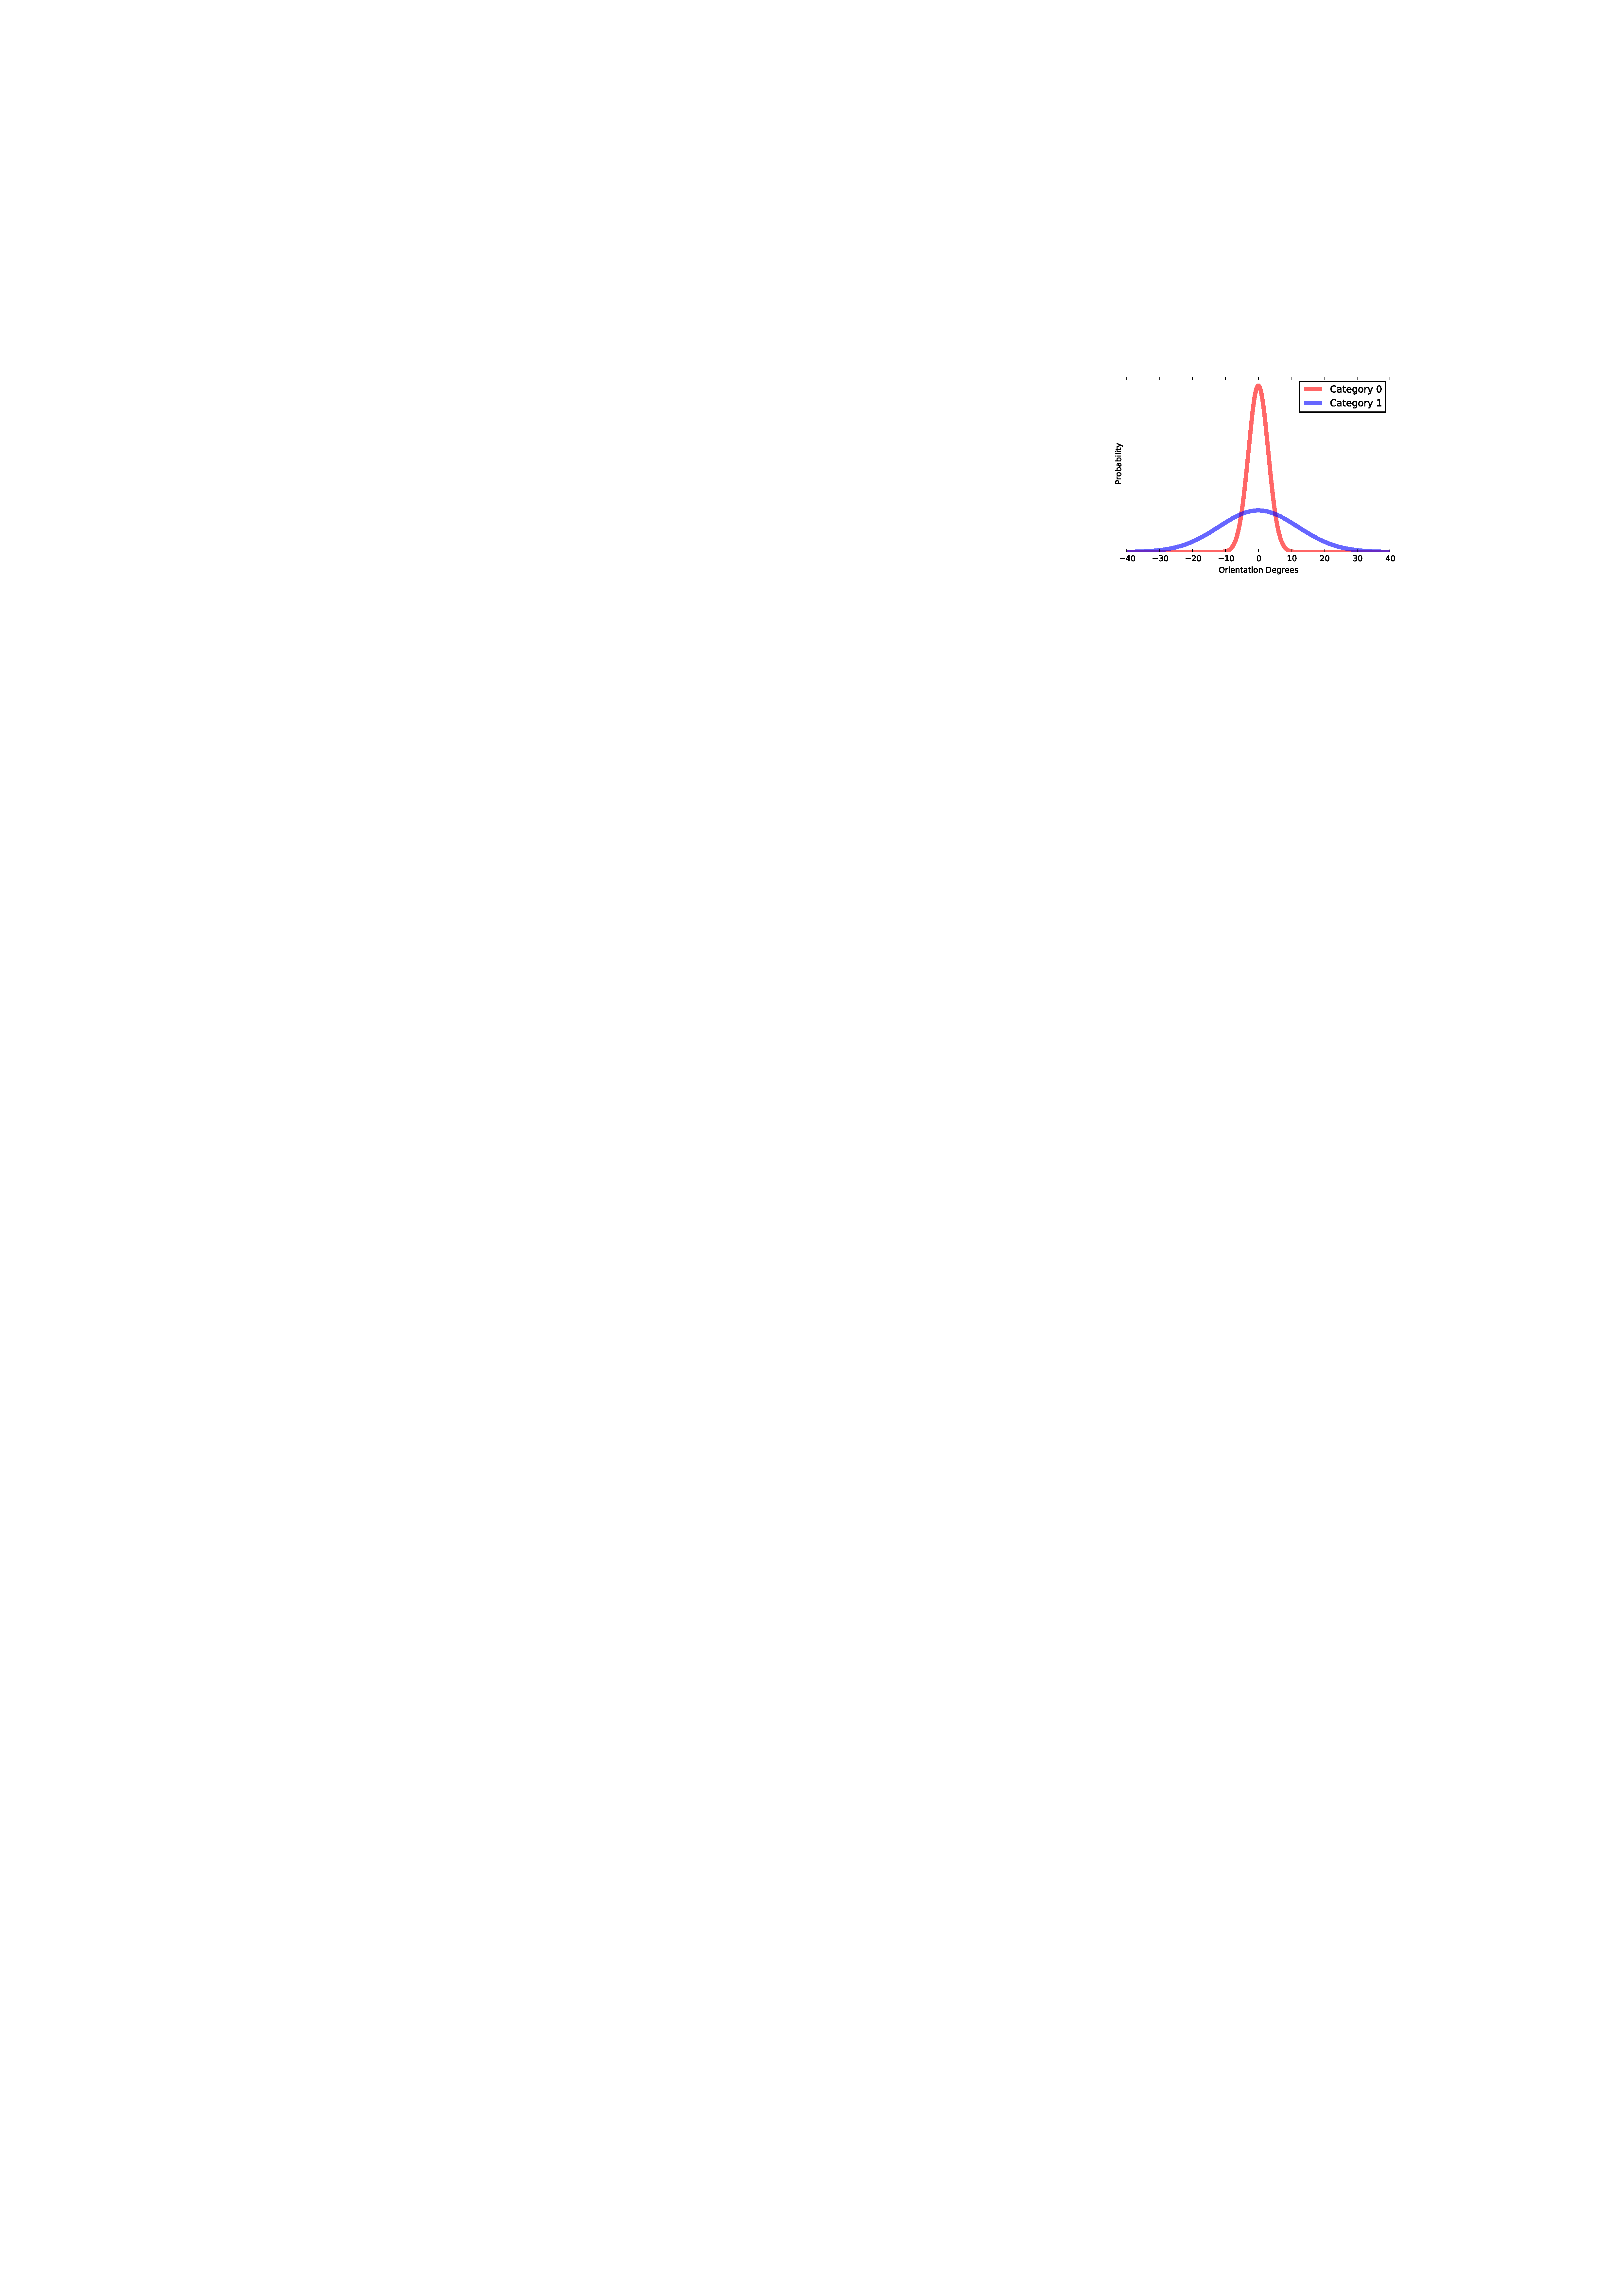
\includegraphics[width = .7\textwidth]{Categorization.pdf}
    \end{column}
  \end{columns}
\end{frame}

\begin{frame}{Previous Work}
  \begin{itemize}
  \item
  	One proposal: variational inference (Beck et al. 2012)
   \begin{itemize}
    \item
    	Assume a parametric form of distributions for approximation and then use coordinate ascent (EM) to minimize KL divergence to true posterior
   \item
   	The coordinate ascent method produces dynamic equations which could be implemented by neurons after a lot of training
  \end{itemize}
    \item
   	Requires analytic derivation of coordinate ascent equations
   \begin{itemize}
    \item
    	No understanding of learning process
  \end{itemize}
     \item
     	Often involves complex nonlinear operations
   \end{itemize}
\end{frame}

\begin{frame}{Approach}
  \begin{columns}[T]
    \begin{column}{.5\textwidth}
  	\begin{itemize}
  	\item
  	Interpret a Deep Neural Net as a generative model (Ranganath et al. 2015)
	\item
	Each layer of neurons corresponds to a layer in the hierarchical distribution
	\item
	Model learns the weights (i.e. how layers are connected) through training	
	\begin{itemize}
		\item
		(In theory)
	\end{itemize}
	\end{itemize}
    \end{column}
    \begin{column}{.5\textwidth}
   	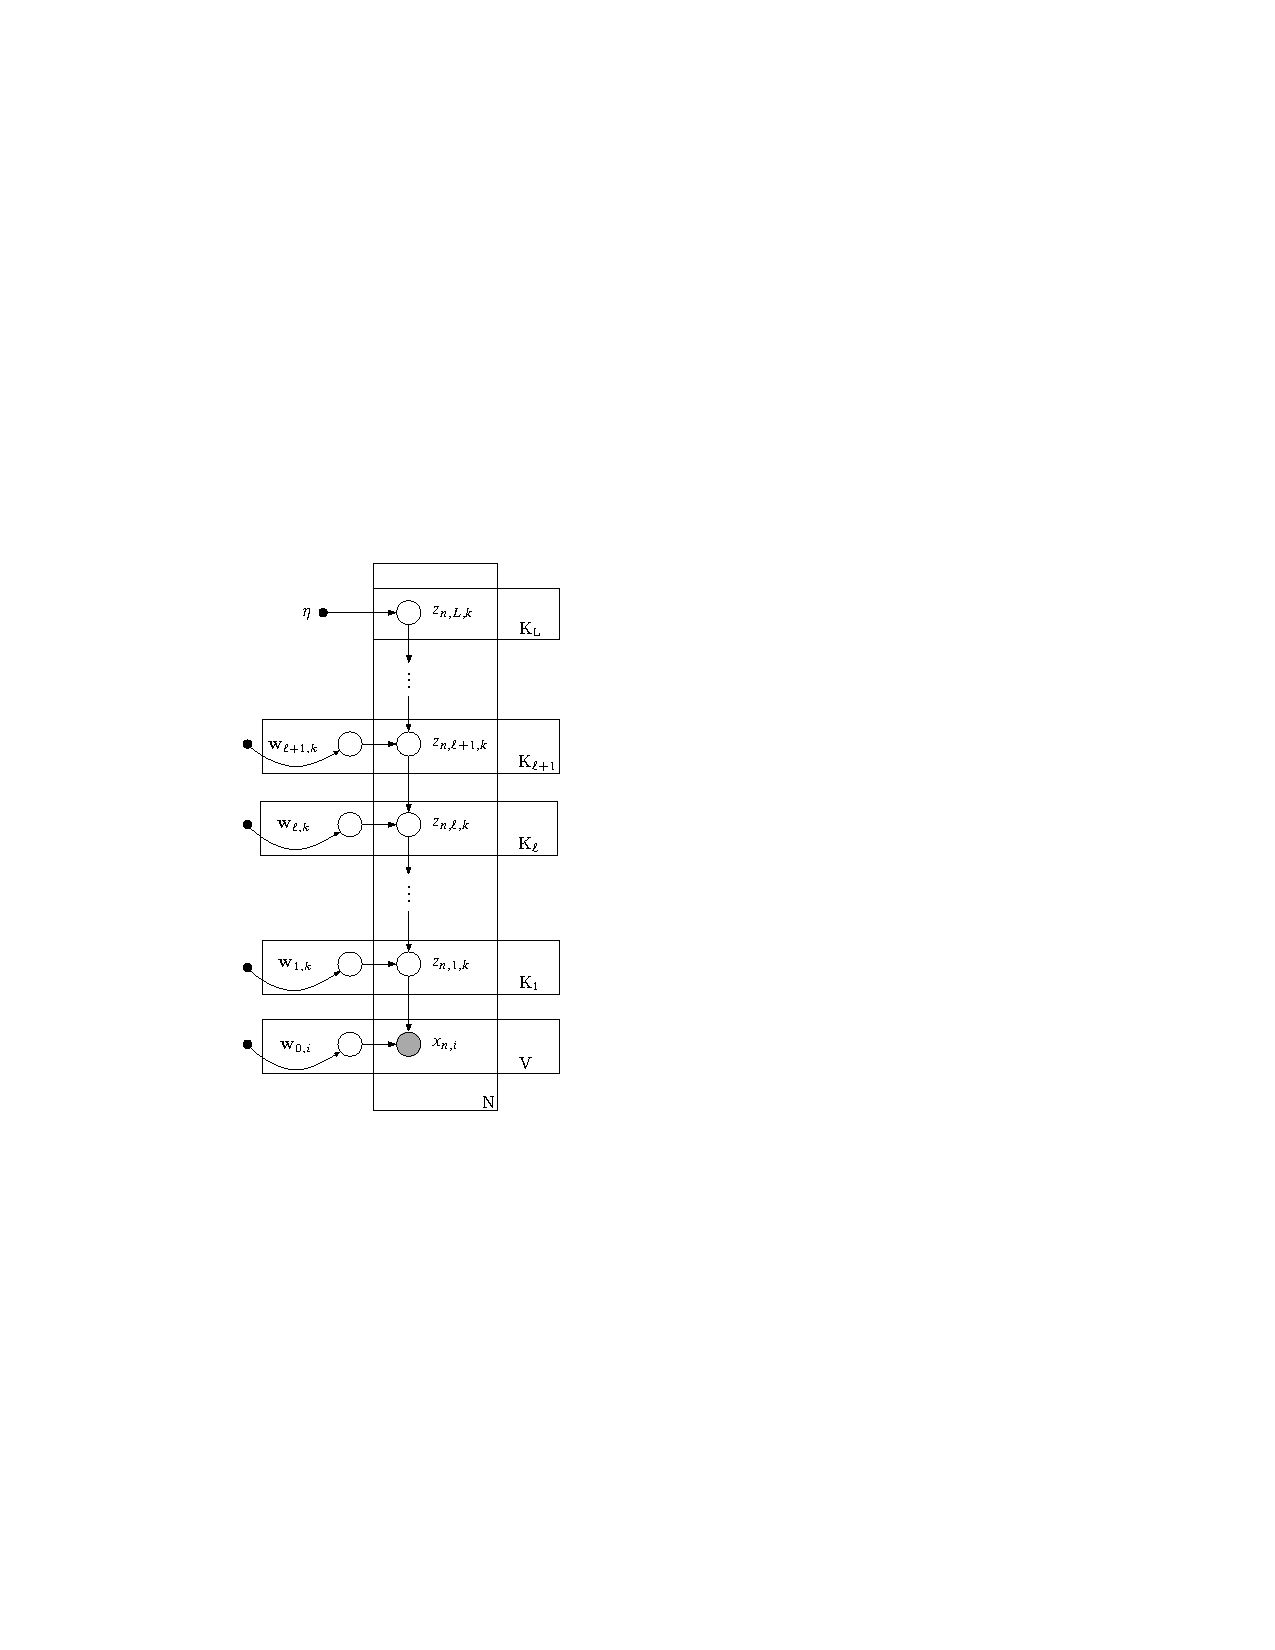
\includegraphics[width = 0.7\textwidth]{DEF.pdf}
    \end{column}
  \end{columns}
\end{frame}

\begin{frame}{Why is this plausible?}
  \begin{itemize}
  \item
  	Requires that neurons sample from exponential family distributions
	\begin{itemize}
  	\item
  		We already model neural noise as exponential family distributions!
	\end{itemize}
  \item
  	Other computations are just linear sums
  \item
  	No need to specify tuning curves of input layer or how to integrate information from input layer
  \item
  	Only uses information from neighboring layers
  \item
  	Algorithm finds closest approximation with arbitrary exponential-family distributions
  \item
  	Caveats
	 \begin{itemize}
	 \item
	 	A lot of reliance on feedback connections
	\item
		Need to be able to semiaccurately modulate mean/variance of synaptic weights/spikes
	\item
		Need to be able to extract mean rate (i.e. integrate) over a number of spikes
  \end{itemize}
  \end{itemize}
\end{frame}

\begin{frame}{Results}
\begin{columns}[T]
    \begin{column}{.5\textwidth}
  \begin{itemize}
  \item
  	...None
  \item
  	Seems to be very difficult to learn distributions
  	\begin{itemize}
	 \item
  		Perhaps due to variational assumption about weights
	 \end{itemize}
  \item
  	Tried simplifying models and smarter learning rates (RMSProp)
  \end{itemize}
  \end{column}
  \begin{column}{.5\textwidth}
   	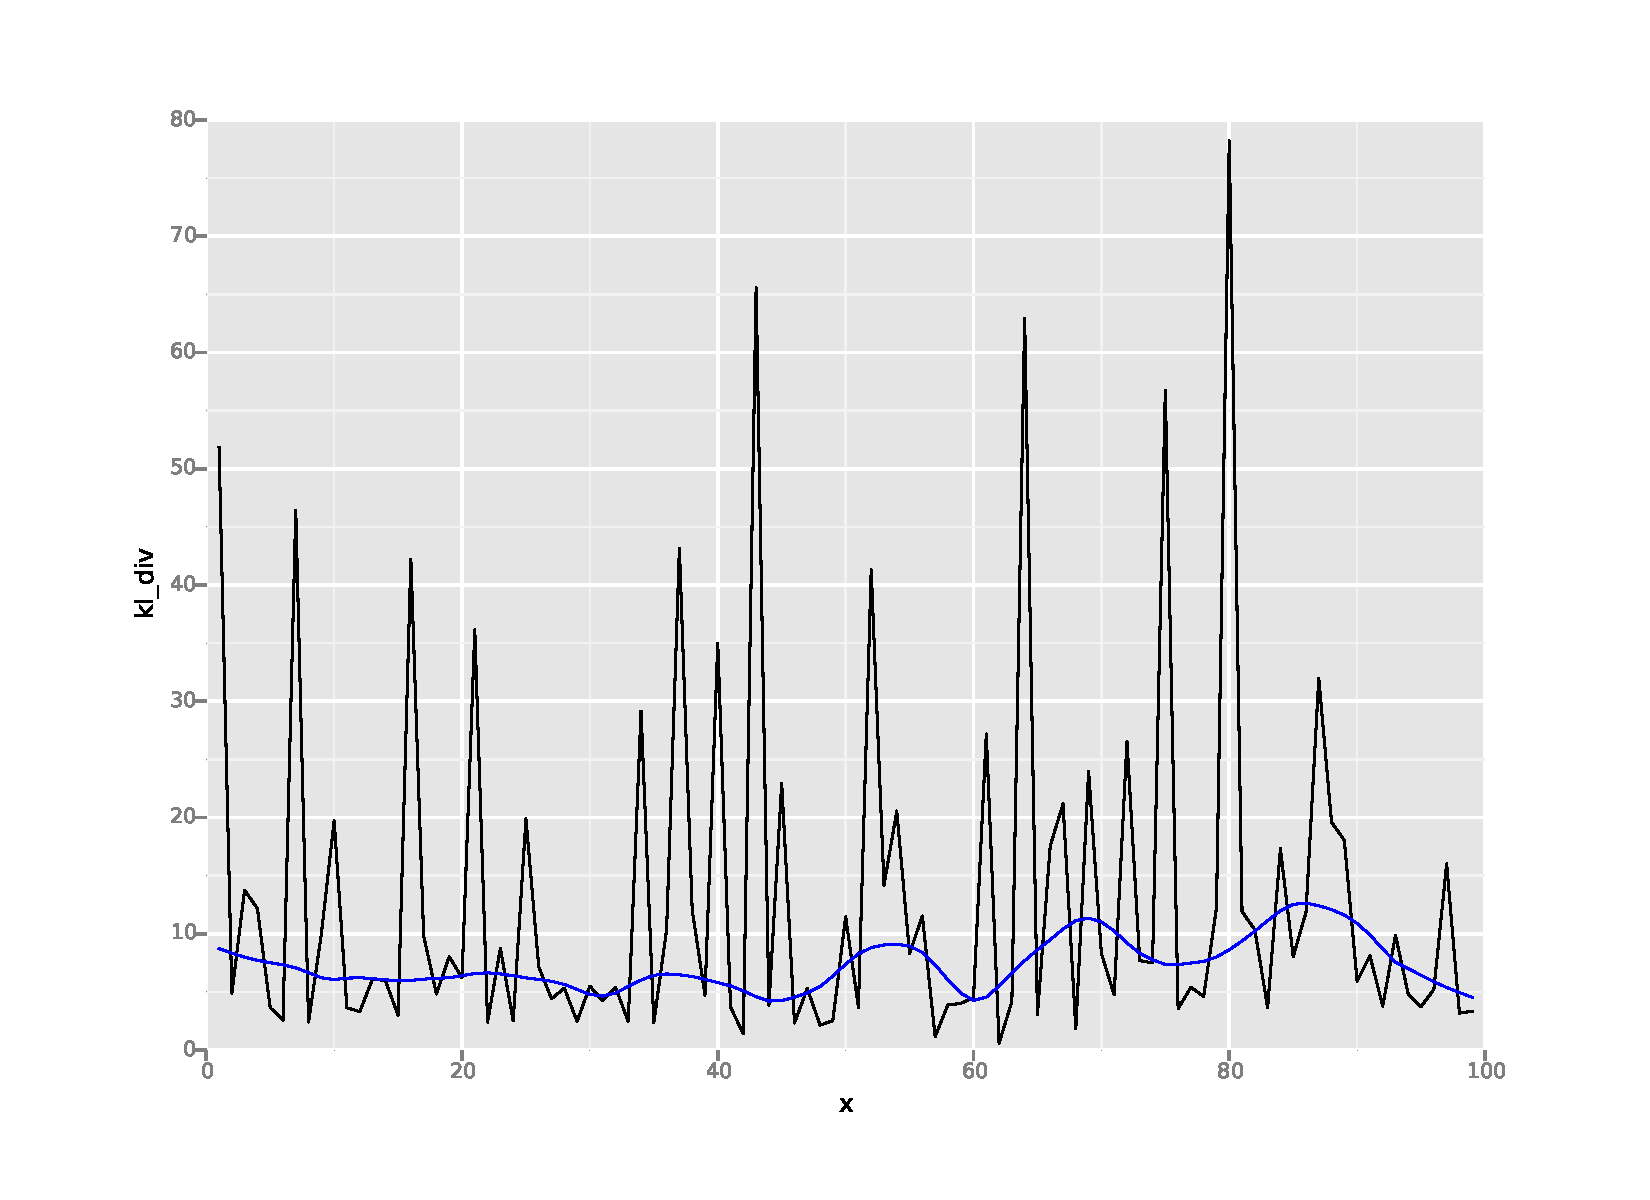
\includegraphics[width = 1\textwidth]{kl.pdf}
    \end{column}
  \end{columns}
\end{frame}

\begin{frame}{Conclusions/Future Work}
  \begin{itemize}
  \item
  	Potentially interesting, more biologically plausible Bayesian inference AND learning
  \item
  	Related to recent work on STDP as gradient descent in variational inference by Bengio et al. (2015)
  \item
  	Future work
  	\begin{itemize}
  	\item
  		Compare to C code posted by authors this weekend
	\item
		Try Bayesian filtering approach to gradient descent updates as in Houlsby and Blei (2014)
	 \end{itemize}	
  \end{itemize}
\end{frame}
\end{document}


